%
% This is the LaTeX template file for lecture notes for EE 382C/EE 361C.
%
% To familiarize yourself with this template, the body contains
% some examples of its use.  Look them over.  Then you can
% run LaTeX on this file.  After you have LaTeXed this file then
% you can look over the result either by printing it out with
% dvips or using xdvi.
%
% This template is based on the template for Prof. Sinclair's CS 270.

\documentclass[twoside]{article}
\usepackage{graphicx}
\usepackage{wrapfig}
\usepackage{amsmath}
\usepackage{amssymb}
\usepackage{listings}
\setlength{\oddsidemargin}{0.25 in}
\setlength{\evensidemargin}{-0.25 in}
\setlength{\topmargin}{-0.6 in}
\setlength{\textwidth}{6.5 in}
\setlength{\textheight}{8.5 in}
\setlength{\headsep}{0.75 in}
\setlength{\parindent}{0 in}
\setlength{\parskip}{0.1 in}

%
% The following commands set up the lecnum (lecture number)
% counter and make various numbering schemes work relative
% to the lecture number.
%
\newcounter{lecnum}
\renewcommand{\thepage}{\thelecnum-\arabic{page}}
\renewcommand{\thesection}{\thelecnum.\arabic{section}}
\renewcommand{\theequation}{\thelecnum.\arabic{equation}}
\renewcommand{\thefigure}{\thelecnum.\arabic{figure}}
\renewcommand{\thetable}{\thelecnum.\arabic{table}}

%
% The following macro is used to generate the header.
%
\lstset{language=Python, numbers=left, tabsize=2, xleftmargin=5.0ex}

\newcommand{\lecture}[4]{
   \pagestyle{myheadings}
   \thispagestyle{plain}
   \newpage
   \setcounter{lecnum}{#1}
   \setcounter{page}{1}
   \noindent
   \begin{center}
   \framebox{
      \vbox{\vspace{2mm}
    \hbox to 6.28in { {\bf EE 382V: Parallel Algorithms
                        \hfill Summer 2017} }
       \vspace{4mm}
       \hbox to 6.28in { {\Large \hfill Lecture #1: #2  \hfill} }
       \vspace{2mm}
       \hbox to 6.28in { {\it Lecturer: #3 \hfill Scribe: #4} }
      \vspace{2mm}}
   }
   \end{center}
   \markboth{Lecture #1: #2}{Lecture #1: #2}
   %{\bf Disclaimer}: {\it These notes have not been subjected to the
   %usual scrutiny reserved for formal publications.  They may be distributed
   %outside this class only with the permission of the Instructor.}
   \vspace*{4mm}
}

%
% Convention for citations is authors' initials followed by the year.
% For example, to cite a paper by Leighton and Maggs you would type
% \cite{LM89}, and to cite a paper by Strassen you would type \cite{S69}.
% (To avoid bibliography problems, for now we redefine the \cite command.)
% Also commands that create a suitable format for the reference list.
\renewcommand{\cite}[1]{[#1]}
\def\beginrefs{\begin{list}%
        {[\arabic{equation}]}{\usecounter{equation}
         \setlength{\leftmargin}{2.0truecm}\setlength{\labelsep}{0.4truecm}%
         \setlength{\labelwidth}{1.6truecm}}}
\def\endrefs{\end{list}}
\def\bibentry#1{\item[\hbox{[#1]}]}

%Use this command for a figure; it puts a figure in wherever you want it.
%usage: \fig{NUMBER}{SPACE-IN-INCHES}{CAPTION}
\newcommand{\fig}[3]{
			\vspace{#2}
			\begin{center}
			Figure \thelecnum.#1:~#3
			\end{center}
	}
% Use these for theorems, lemmas, proofs, etc.
\newtheorem{theorem}{Theorem}[lecnum]
\newtheorem{lemma}[theorem]{Lemma}
\newtheorem{proposition}[theorem]{Proposition}
\newtheorem{claim}[theorem]{Claim}
\newtheorem{corollary}[theorem]{Corollary}
\newtheorem{definition}[theorem]{Definition}
\newenvironment{proof}{{\bf Proof:}}{\hfill\rule{2mm}{2mm}}

% **** IF YOU WANT TO DEFINE ADDITIONAL MACROS FOR YOURSELF, PUT THEM HERE:

\begin{document}
%FILL IN THE RIGHT INFO.
%\lecture{**LECTURE-NUMBER**}{**DATE**}{**LECTURER**}{**SCRIBE**}
\lecture{19}{July 21}{Vijay Garg}{Abed Haque}
%\footnotetext{These notes are partially based on those of Nigel Mansell.}

% **** YOUR NOTES GO HERE:

% Some general latex examples and examples making use of the
% macros follow.  
%**** IN GENERAL, BE BRIEF. LONG SCRIBE NOTES, NO MATTER HOW WELL WRITTEN,
%**** ARE NEVER READ BY ANYBODY.
\section{Introduction}
During this lecture we covered the following topics:

\begin{itemize}
	\item The Maximal Independent Set (MIS) Problem
	\item Luby's Algorithm
\end{itemize}

This set of lecture notes will briefly re-examine the topics covered in this lecture, in the order in which they appeared during class. 

\section{The Maximal Independent Set Problem}
Suppose that we are given an undirected graph, \textit{G = (V, E)}.  A set of vertices $V'\subseteq V$ is said to be \textit{independent} if there is no edge between any two vertices \textit{V'}.  There can be many independent sets.
\begin{figure}[!ht]
\centering
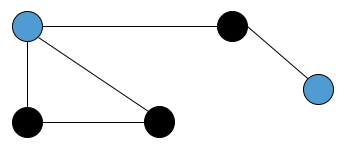
\includegraphics[scale=0.7]{img/IndependentSet.png}
\caption{A possible independent set (blue vertices)} \label{fig:indSet} 
\end{figure}

An independent set is considered to be \textit{maximal} if there is no independent set that strictly contains \textit{V'}. Figure \ref{fig:indSet} is maximal since no other vertex can be added to {V'} while still being an independent set.  The largest possible maximal independent set is called a \textit{maximum} independent set.  Finding the maximum independent set is NP-hard, so we will only focus on how to find maximal independent sets instead.

\clearpage
\subsection{Greedy Sequential Algorithm For MIS}

\begin{lstlisting}[mathescape=true]
$I := \emptyset$// Start with an empty independent set
for $v:=1$ to n do
	if $I \cap T(v) = \emptyset $ then
    	$I := I \cup \left\{v\right\}$
\end{lstlisting}

$T(v)$ represents the neighbors of $v$. This has a time complexity of \textit{O(n)}. 

\section{Luby's Algorithm}
Luby's algorithm is a randomized parallel algorithm to find the maximal independent set.  The input is a graph $G = (V, E)$ and the output is the independent set $I$.  The steps are as follows:

\begin{lstlisting}[mathescape=true,numbers=none]
1. $I := \emptyset$
2. repeat
	2.1 for all $v \in V$ in parallel do
				if (d(v) = 0) then add v to I and delete from V   //corner case
				else mark v with probability $1/(2d(v))$
 	2.2 for all $(u,v) \in E$ do in parallel
    			if both u and v are marked then unmark the lower degree vertex
 	2.3 for all $v \in V$ in parallel
    			if v is marked then add v to S; // S is the vertices in this iteration
	2.4 $I := I \cup S$  
	2.5 delete $S \cup T(S)$ from V and all incident edges to $S \cup\ T(s)$ until $V = \emptyset$
\end{lstlisting}

Intuitively, the nodes with fewer neighbors will be able to add more nodes.  Above, $d(v)$ represents the degree of $v$. When $d(v)$ is large, there are lots of neighbors, and we can say that they are rich (socially).  The richer the vertex, the smaller its probability of being marked is.  Once the entire graph is empty we're done.

Each step of this algorithm is done in constant time, in parallel.  We want to show that in log(n) iterations that we'll be done (with a high probability).

A vertex $v \in V$ is known as a \textit{good vertex} if it has at least $d(v)/3$ neighbors of degree no more than $d(v)$.  A vertex is \textit{bad} if it is not \textit{good}.  An edge is \textit{good} if at least one of its endpoints is a good vertex.

\subsection{Overall Strategy}
1.  There is a constant probability of a good vector being deleted

2.  There are a large number of good edges.  If a constant fraction of good edges are deleted \textit{and} good edges form a constant fraction of total edges, then a \textit{constant fraction} of all edges gets deleted in every iteration.  If the number of edges are reduced by a factor of 2 every time, it will take $log_2n$ iterations.  If we reduce the number of edges by a factor of 100 every time, it will take $log_{100}n$ iterations.  (But we really don't care because its $O(log(n))$.

This parallel algorithm was a breakthrough!

\clearpage
\subsection{Proofs}
Let's prove part 1 of the overall strategy.

Lemma:  Let $v \in V$ be a good vertex with degree $d(v) > 0$.  the probability that some vertex $w \in \Gamma (v)$ gets marked with at least $1 - e^{-1/6}$.

Proof: If $v$ is good $\Rightarrow $ there are at least $d(v)/3$ neighbors with degree at most $d(v)$

1.  The probability of one of these neighbors not being marked is $\leq 1 - 1/(2d(v))$


2. The above is independent, therefore we can multiply probabilities.  The probability that none of these neighbors are marked is at most $\leq (1 - 1/(2d(v)))^{d(v)/3} \leq e^{-1/6}$


Let's bring some special attention to this last inequality, as it is very simple, but perhaps the most useful inequality in randomized algorithms.

\begin{center}
$1 + x \leq e^x $ for all $x$
\end{center}

\begin{figure}[!ht]
\centering
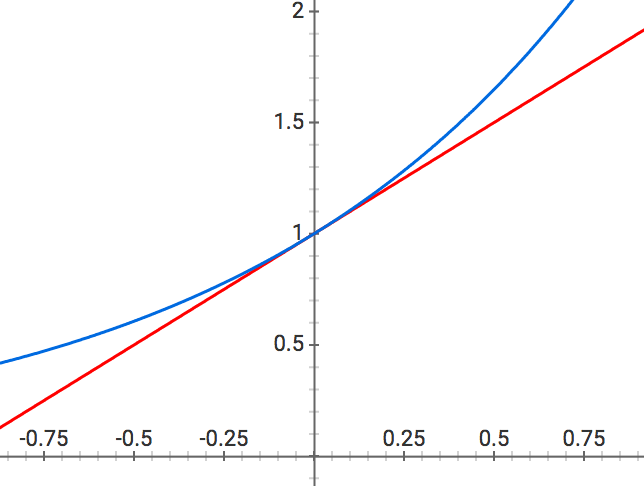
\includegraphics[scale=0.7]{img/inequality.png}
\caption{$y = e^x$ (blue) and $y=1+x$ (red)} \label{fig:inequality} 
\end{figure}

Now back to the proof.  Let's first multiply the exponent portion of the probability by 2:

\begin{center}
$(1 - 1/(2d(v)))^{2d(v)/6} \leq e^{-1/6}$
\end{center}

Now let's use the above inequality and substitute.

\begin{center}
$(1 - 1/x)^{x} \leq e^{-1}$
\end{center}

By substitution $n=2d(v)$ we get the desired result:

\begin{center}
$(e^{-1})^{1/6} < e^{-1/6}$
\end{center}

We have shown constant probability of getting marked!  Now let's show that the probability of getting \textit{unmarked} is also constant.

Lemma:  During any iteration, if a vertex v is marked, then it is selected to be in $S$ with a probability of at least $1/2$.

Proof:  The vertex $w$ is not selected only if one of its neighbors with degree $\geq d(w)$ is also marked.  Each such neighbor is marked with probability $\leq 1/(2d(w))$.  By union bound, the probability that a marked vertex is selected to be in $S$  is $\leq \sum_{v} (1/(2d(w)) = 1/2$.

Lemma:  In a group $G(V,E)$, the number of good edges is at least $|E|/2$ 

Proof:  A vertex is bad if at least 2/3 of its neighbors are richer.  Direct the edges from a lower degree end-point to a higher degree endpoint.

\begin{center}
$d_o(v) - d_i(v) \geq d(v)/3 = (d_o(v) + d_i(v))/3$
\end{center}

Now let's sum everything.  The total degree of bad vertices  is equal to 
\begin{center}
$2e(V_B, V_B) + e(V_B, V_G) + e(V_G, V_B)$
\end{center}

The first term indicates edges going from $V_B$ to $V_B$ and thus are counted twice.  This can be rewritten as:
\begin{center}
$= \sum\limits_{v \in V_B} (d_o(v)  + d_1(v))$
\end{center}

Now let's use the inequality from before:
\begin{center}
$\leq 3\sum\limits_{v \in V_B} (d_o(v)  - d_1(v))$

$= 3(e(V_B, V_G) - e(V_G, V_B))$

$\leq 3(e(V_B, V_G) + e(V_G, V_B))$
\end{center}

Resulting in:

\begin{center}
$e(V_B, V_B) \leq e(V_B, V_G) + e(V_G, V_B)$
\end{center}

This is saying that edges going from bad to bad are one less than good edges.  Bad edges $\leq$ good edges implies that good edges $\geq |E|/2$, which is what we were trying to show.

Now we have a theorem that says that since a constant fraction of the edges are on good vertices, and good vertices get eliminated with a constant probability, the expected number of edges eliminated during an iteration is a constant fraction of the current set of edges.  If a vertex gets marked, they will stay marked with a probability of 1/2.

\clearpage
\section{Euler Tour Technique}
Given some tree, let's say that we want to find the height of the tree.  If it was a balanced tree, this would be easy to do.  But what if the tree was skewed?  The height may not be $log(n)$ in this case.  The Euler Tour Technique is a way to find the height of a tree in $log(n)$ time independent of the height.

Let's think of a linked list as a lopsided tree.  With pointer jumping, we were able to find the length of the linked list in $log(n)$ time.  We can use a similar technique for a tree if we represent it as a linked list.

Given a directed graph, a Euler Tour is a walk along the edges of the graph, starting from any node $v$, in which every edge is traversed exactly once and ends at the vertex $v$.  A graph has an Euler Circuit if and only if every node has an even degree (an even number of edges).

We can view a tree as a linked list of edges.  Let's construct a directed graph from a tree and then define a Euler Tour for the graph.  It is sufficient to specify  the next edge (successor) for every edge $e$ in the directed graph.  Let $v_0 , v_{m-1}$ be the neighbors of $u$.  Then $succ(v_i, u)$ is given by $(u, v_{(i+1\enspace mod\enspace m)})$.  (This is depth first search).

\subsection{Implementation of Euler Tour on a Graph from a Tree} 

Given the tree T shown in Figure \ref{fig:euler1} below, we will construct a Euler Tour.  Figure \ref{fig:euler2} shows the adjacency list representation of the T.  Now let's make two modifications to Figure \ref{fig:euler2}.  First, lets make the lists circular instead of null terminating.  Second, lets put a bidirectional pointer between edges that represents the same undirected edge, represented by a blue dotted line.  This results in the circular adjacency list in Figure \ref{fig:euler3}. 

In this example $succ(1,4) = (4,2)$.  In Figure \ref{fig:euler3}, $succ$ is the element that is shown by the blue dotted edges followed by black edges.  So we can can construct the following Euler Tour directly from Figure \ref{fig:euler3}:

$(1, 4) \rightarrow (4, 2) \rightarrow (2, 4) \rightarrow (4, 3) \rightarrow (3, 4) \rightarrow (4, 1) \rightarrow (1, 5) \rightarrow (5, 1) \rightarrow (1, 4)$

\begin{figure}[!ht]
\centering
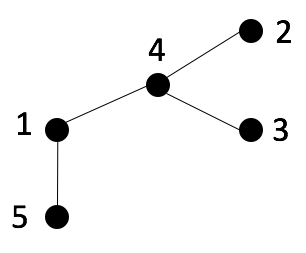
\includegraphics[scale=0.6]{img/EulerCkt1.png}
\caption{A tree T} \label{fig:euler1} 
\end{figure}

\begin{figure}[!ht]
\centering
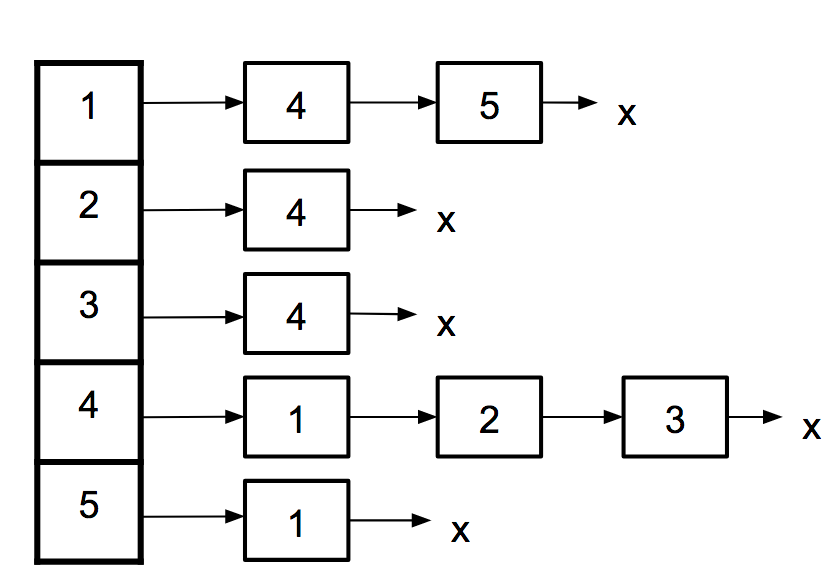
\includegraphics[scale=0.4]{img/EulerCkt2.png}
\caption{The adjacency lists of the tree T} \label{fig:euler2} 
\end{figure}

\begin{figure}[!ht]
\centering
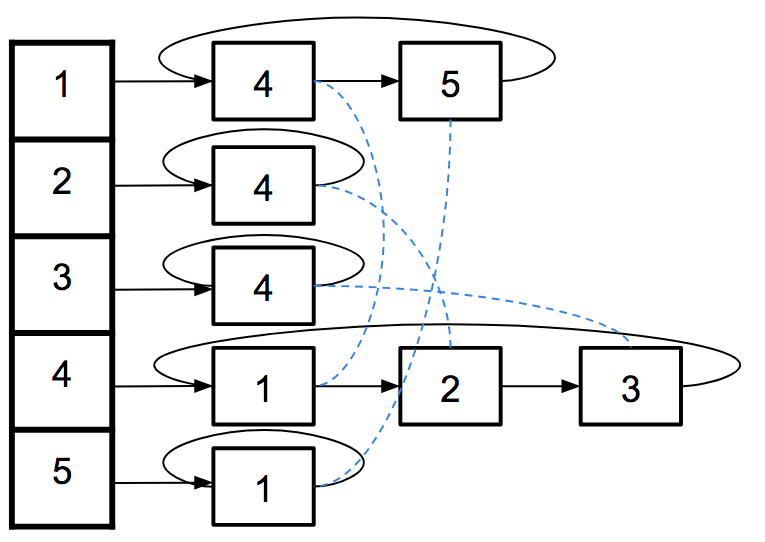
\includegraphics[scale=0.4]{img/Euler3.png}
\caption{The circular adjacency lists of tree T with additional pointers} \label{fig:euler3} 
\end{figure}

\end{document}



Contact GitHub API Training Shop Blog About
� 2017 GitHub, Inc. Terms Privacy Security Status Help